\documentclass[10pt,conference,compsocconf]{IEEEtran}

\usepackage{hyperref}
\usepackage{graphicx}	% For figure environment
\usepackage{amsmath}
\usepackage{amssymb}
\usepackage{float}
\usepackage{url}
\newcommand{\beginsupplement}{%
	\setcounter{table}{0}
	\renewcommand{\thetable}{S\arabic{table}}%
	\setcounter{figure}{0}
	\renewcommand{\thefigure}{S\arabic{figure}}%
}

\begin{document}
\title{Extreme Wind Analysis}

\author{
	Matthias Minder, Yves Rychener
}

\maketitle


\begin{abstract}
Modeling extreme conditions has many applications in Finance, Insurance, Environment and others. In this article we report the results of our analysis on the extreme weather conditions leading to extreme thunderstorms in central Kansas in the United States using various approaches. As expected, we consistently discover a seasonality, showing that thunderstorms are much more extreme during summer months. Moreover, during all months except December, there is not enough evidence to support a time-dependence. Interestingly, in the month of December extreme thunderstorms seem to significantly decrease in severeness over the course of time. Finally, we provide estimated return levels for every month, which could be valuable for risk assessment in insurance. 
\end{abstract}

\section*{Introduction} 
Modeling extreme weather events is of interest for a variety of applications, such as risk assessment for insurance companies or conception of preventive measures. In particular, questions about how often a particular event will occur, how severe events can get, and whether there are seasonal or year-dependent trends are of interest. Within the scope of this report, we will address these questions for extreme thunderstorms on a 1° longitude and 1° latitude grid cell with south-west coordinates 38° latitude and -100° longitude, situated in central Kansas. The measured quantities are the Connective Available Potential Energy ($CAPE$) and the Storm Relative Helicity ($SRH$), which have to be simultaneously high for severe thunderstorms to occur. Three-hourly time series of these events are taken into account from January 1st 1979 at 00:00 to December 31st 2015, 21:00. 
\par
In particular, we will study the structure variable denoted $PROD$ given by $PROD = \sqrt{CAPE} \times SRH$. It captures concurrently high values of $SRH$ and $CAPE$, and is thus apt for modeling the risk of thunderstorms. Every month will be treated separately in order to capture seasonal differences. To model extreme values, a generalized extreme value distribution will be fitted to the monthly maxima of $PROD$ using maximum likelihood estimation as well as Bayesian approaches. Moreover, the generalized extreme value distribution will be fitted to the $r$-largest order statistic for every month to determine whether that improves the fit. Subsequently, we will assess dependence of $PROD$ upon time and the NINO 3.4 index, an established indicator of the El-Niño Southern Oscillation ($ENSO$). 
\par
Following this, $CAPE$ and $SRH$ are considered separately. We will study whether they are asymptotically dependent, before fitting bivariate models to the joint extremes of $CAPE$ and $SRH$. 
Finally, 50- and 100-year return levels of $PROD$ are calculated based on fitting a point process model to $PROD$ with maximum likelihood estimation, based on the Bayesian fit, and based on simulated values of $CAPE$ and $SRH$ from the bivariate model fitted before. 

\section*{Preliminary Analysis}
\begin{figure}
	\centering
	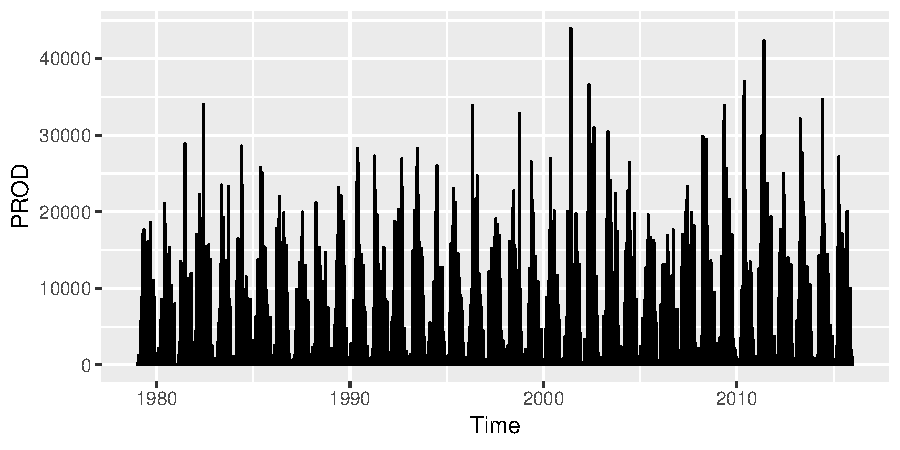
\includegraphics[width=0.35\textwidth]{../plots/full_time_series.pdf}
	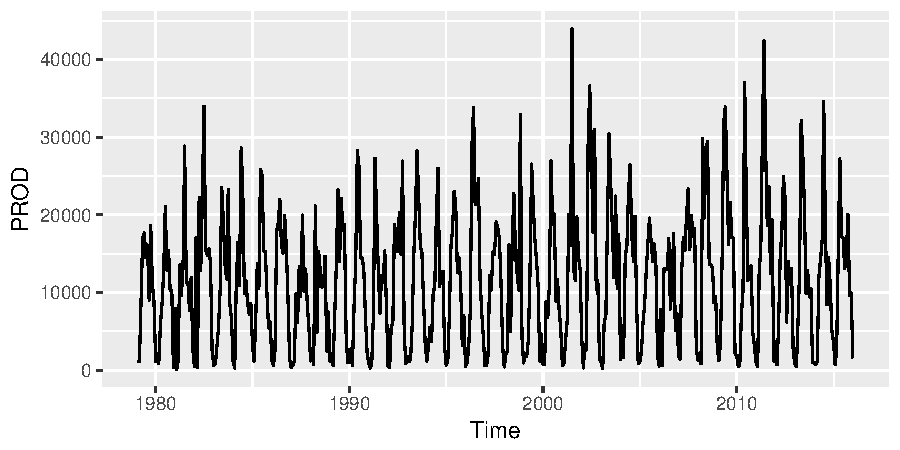
\includegraphics[width=0.35\textwidth]{../plots/monthly_max_series.pdf}
	\caption{Three-hourly values (top) and monthly maxima (bottom) of $PROD$ values for the entire analyzed period.}
	\label{fig:timeseries}
\end{figure}
Plotting the full time series and the monthly maxima as shown in Figure \ref{fig:timeseries} clearly shows the seasonality of the data, with high values of $PROD$ occurring mainly during summer. This clearly shows the necessity of separate treatment of months. Moreover, there seems to be some upward trend following time, with more extreme values of $PROD$ in recent years.

\section*{Fitting Generalized Extreme Value Distribution to PROD}
In order to understand the behavior of the monthly maxima, we fitted a generalized extreme value (GEV) distribution to $PROD$ for each month separately with three different approaches. 
\begin{figure}
	\centering
	\textbf{January}\\
	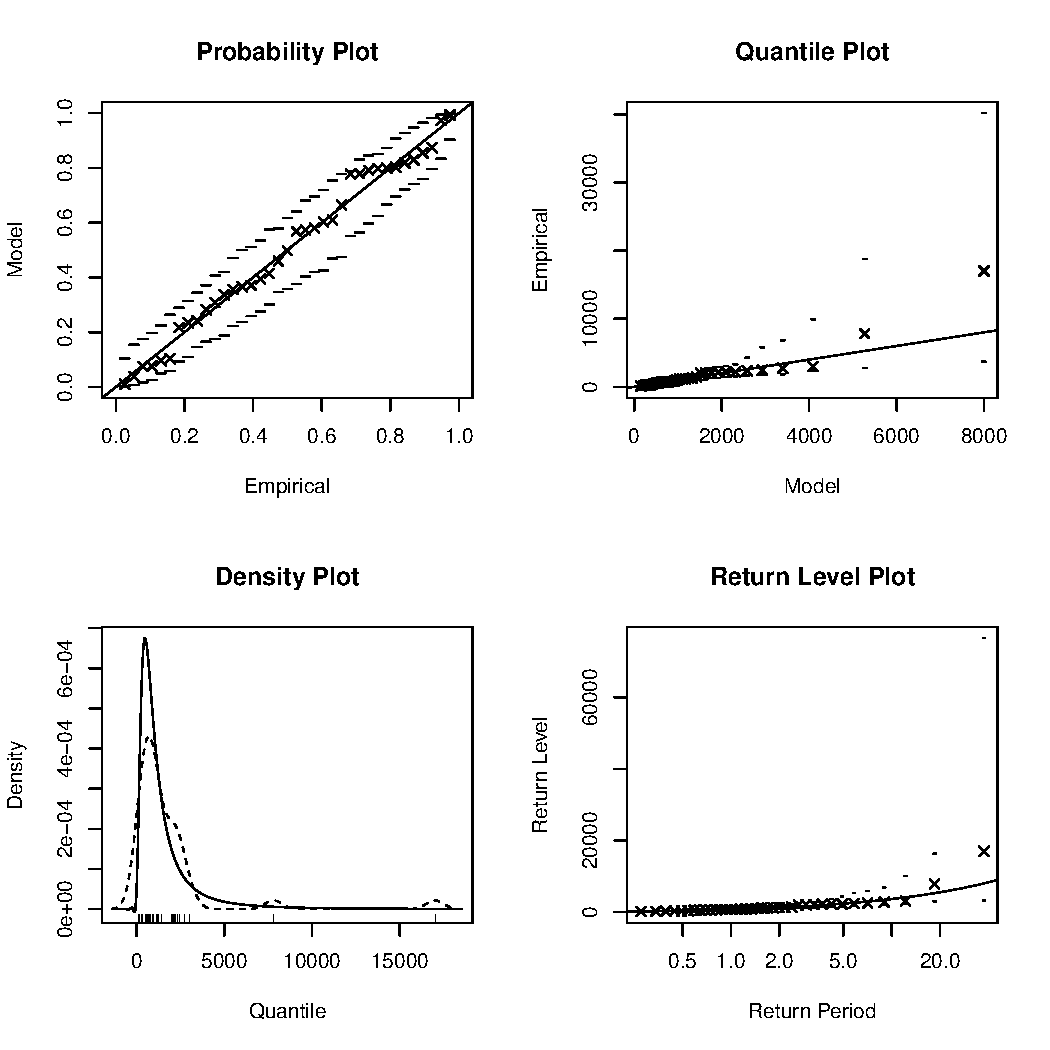
\includegraphics[width=0.35\textwidth]{../plots/monthly_mle_diag/01_monthly_mle_diag.pdf}\\
	\textbf{December}\\
	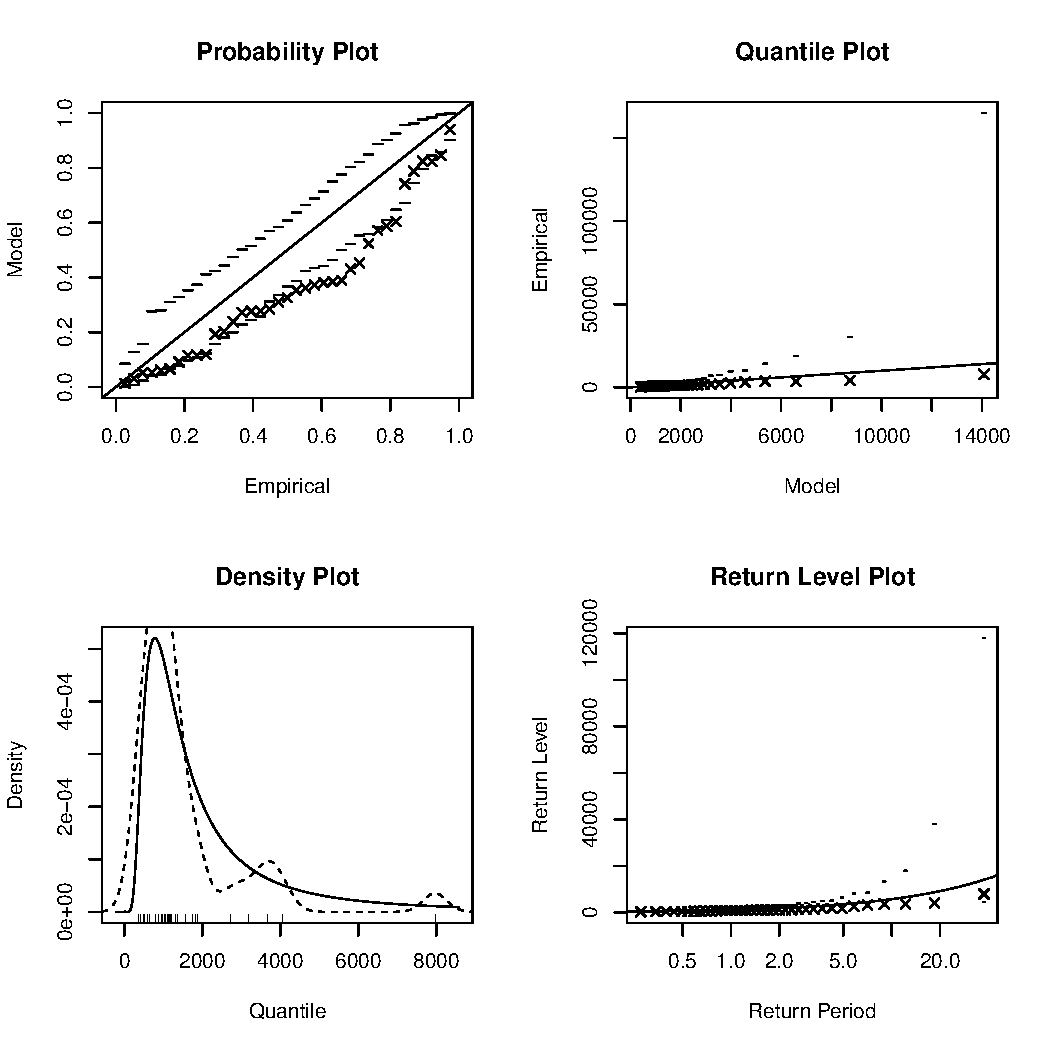
\includegraphics[width=0.35\textwidth]{../plots/monthly_mle_diag/12_monthly_mle_diag.pdf}
	\caption{Diagnostic plots for fitting GEV to the data using maximum likelihood estimation for January (top) and December (bottom). Whereas in January the model fits the data, as shown by the fact that the observed values are within the confidence range for probability plot, this is not the case for December, indicating a poor fit.}
	\label{fig:mle_diag}
\end{figure}
\par
First, we fitted the values using maximum likelihood estimation (MLE). Fitting was done using the evd package in R, using the Nelder-Mead optimization method and standard parameters \cite{evd}. The quality of the fit was assessed using diagnostic plots, as shown for January and December in Figure \ref{fig:mle_diag}. The model performed well with the exception of September and December: In September optimization didn't succeed, whereas in December the observed values lie outside of the given confidence intervals, as shown in Figure \ref{fig:mle_diag}. For both of these months, no standard error could be calculated due to singularity of the observed Fisher information matrix. Since we expect some continuity over the course of the year, the problem wasn't further investigated as inferences for the missing months can be made from their adjacent months. 
\par
Then, we fitted the values using the Metropolis-Hastings algorithm. As a prior for the three parameters, a normal distribution with mean zero and a diagonal covariance matrix was used.
Here, we will give an intuitive explanation of the Metropolis-Hastings algorithm; for a more detailed and mathematically rigorous explanation, please refer to slides 82-86 of the course slides.
This algorithm creates a Markov chain with stationary distribution $\pi(x)$, where $\pi(x)$ is also the desired distribution of the parameters of our model. The transition probability from $x$ to $y$ is $p(x,y)=\alpha(x,y) q(x,y)$, where $\alpha(x,y)$ is the acceptance rate, and $q(x,y)$ is the proposition density. We can select the proposition density $q(x,y)$ ourselves, usually a normal distribution is chosen, the acceptance rate can be shown to be $\alpha(x,y)=min(\frac{\pi(y) q(y,x)}{\pi(x) q(x,y)},1)$.
\par
We can imagine the sampling as follows: An agent is navigating the Markov chain. At every iteration, it will sample a proposed step to take from the distribution $q(x,y)$. Then, with probability $\alpha(x,y)$, it is allowed to take said step and move to a new state. With probability $1-\alpha(x,y)$, the step is rejected and we stay at the current state. We can estimate the (unknown) stationary distribution of the chain by navigating $n$ iterations and keeping track of the empirical state distribution. As $n \to \infty$ (or in practice for big $n$), we converge to the true stationary distribution. The proposal standard deviation dictates how big the proposal steps are. If the agent wants to take steps that are too big, he gets rejected all the time and cannot explore the chain. If the proposal steps are too small, he cannot fully explore the chain since $n$ has to be finite in order to finish our calculation. In practice, we have to remove some "burn in", since we may start very far away from the stationary distribution. Also, thinning is applied, since each state is dependent on the preceding state, resulting in high autocorrelation. 
\par
The proposal standard deviations were fine-tuned to obtain acceptance rates between 0.2 and 0.4. In order to avoid having to fine-tune every month separately, we implemented the following very simple optimization algorithm: If the acceptance rates for a given parameter were too high, the proposal standard deviation for said parameter were multiplied with 1.5. In the opposite case for low acceptance rates, the proposal standard deviation was divided by 2. The Metropolis-Hastings algorithm was run with 30'000 iterations. The chain was thinned with a factor 300 in order to avoid dependence between steps of the Markov chain. The thinning was validated with autocorrelation plots (not shown). The final parameter was determined to be the median of the posterior distribution, in order to be robust to outliers and be more adapted to skewed distributions. 
\par
\begin{figure}
	\centering
	\textbf{May}\\
	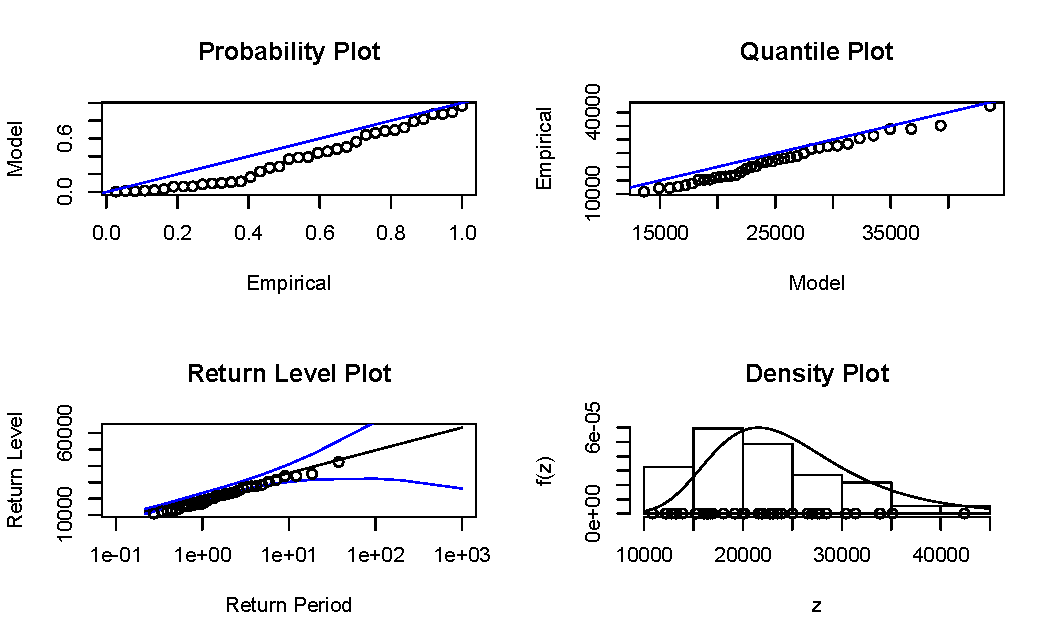
\includegraphics[width=0.35\textwidth]{../plots/r_larg_diag_may.pdf}\\
	\textbf{July}\\
	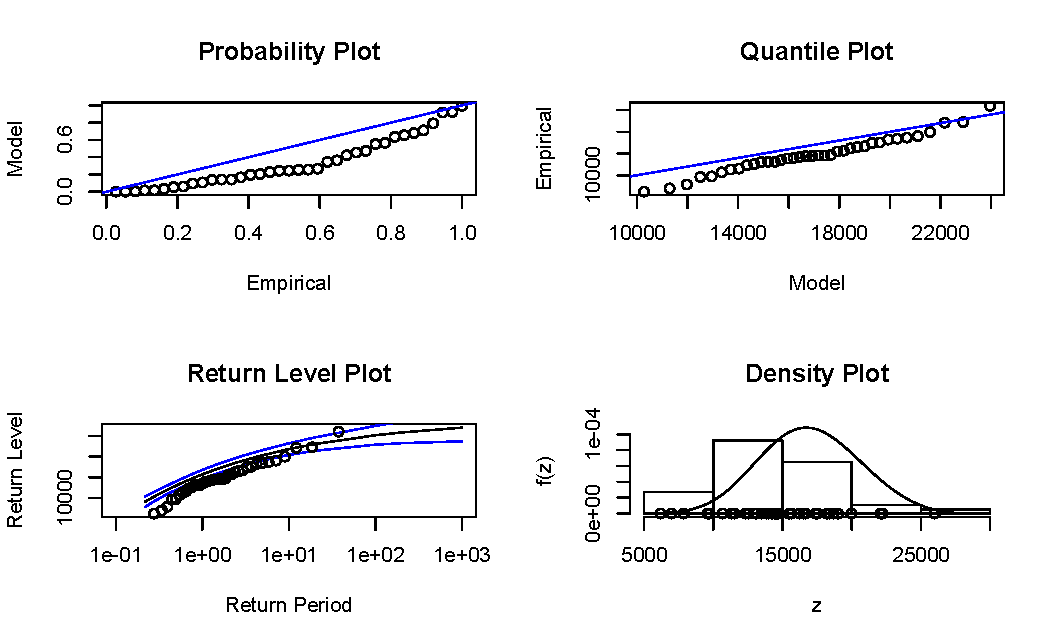
\includegraphics[width=0.35\textwidth]{../plots/r_larg_diag_july.pdf}
	\caption{Diagnostic plots for fitting r-largest-order statistic for January (top) and December (bottom). Whereas in may the model fits the data very well, as shown by the fact that the observed values are within the confidence range for return level plot, this is not the case for July, indicating a poor fit. Also the probability plot indicates a better fit in May.}
	\label{fig:r_diag}
\end{figure}
We then investigated how taking into account the $r$-largest values for every month affects the fit. For fitting the $r$-largest order statistic, we have to find the best $r$ first. This was done by comparing the different parameter standard deviations and MLE deviances: When taking into account $r$ largest values, the standard deviation for all parameters is expected to be reduced by a factor $\sqrt{r}$ with respect to the model using only maxima. If it is reduced by less, this suggests that the additional order statistics don't bring important information and thus don't improve the fit. Similarly, the deviance is expected to be reduced when using more data. However, if this reduction of deviance is small, this again suggests that the additional order statistics don't improve the data. Using these paradigms, we found a reasonable choice to be $r=2$. This choice was confirmed using the diagnostic plots (Figure \ref{fig:r_diag}), which indicated a good fit for all months with exception of July. In Figure \ref{fig:r_diag}, we show the diagnostic plots for May to exemplify a good fit and July to show it's poor fit. 

\section*{Dependence of PROD on Time and ENSO}
A dependence test of $PROD$ on a factor $x$ can be done by likelihood ratio test. Within the scope of this analysis, dependence on time and ENSO as determined by the NINO 3.4 index is assessed. Before fitting the linear trend, we center and renormalise the influencing factor with respect to its mean and standard deviation as recommended in the \texttt{fgev} help files. We tested for linear dependence to account for gradual regime changes, and for a step function dependence centered at the factor mean to allow for rapid changes. More formally, the linear dependence is modeled
\begin{align*}
	\eta(x_{norm}) = \eta_0 + \eta_1*x_{norm}
\end{align*}
while the step change is modeled as 
\begin{align*}
	\eta(x_{norm}) = \begin{cases} \eta_0+\eta_1 & \textrm{if } x_{norm}>0\\ \eta_0 & \textrm{otherwise} \end{cases}
\end{align*}
The test was formulated such that the model with constant $\eta$ is the null hypothesis, and the model with factor-dependent $\eta$ is the alternative hypothesis. We employ the Bonferroni multiple testing method to take into account the multiple tests at 95\% significance level arising from the different months tested. 
\par
Figure \ref{fig:dependance_test} displays the different ratios and the 95\% significance level (red) for linear dependence. We observe that independence with respect to ENSO is rejected in October, while independence with respect to time is rejected in December. For all other months, the null hypothesis cannot be rejected for a significance level of 95\%. Moreover, Figure \ref{fig:dependence_test_step} shows the likelihood ratio and 95\% significance level (red) for step dependence. Here, independence with respect to time is only rejected in December, while the null hypothesis is retained in all other months, and when testing for independence with respect to ENSO. 
\par
It is interesting that the month of December is consistently determined to be time dependent, whether that dependence has a linear or step-function shape, while all other months are determined to be time independent. Moreover, contrary to expectation, the detected linear trend is negative. This suggests that thunderstorms have been getting less severe in December in recent years at the particular location of our measured data. However, this conclusion is based on very little data, and only applies to a single location. More thorough analysis should be done before drawing conclusions from this results. Dependence on ENSO is determined to be of linear nature in October, whereas a step function doesn't sufficiently capture this change. Moreover, since the slope parameter is positive, this suggests that El Niño oscillations positively affect the thunderstorm activity in October. 

\begin{figure}
	\centering
	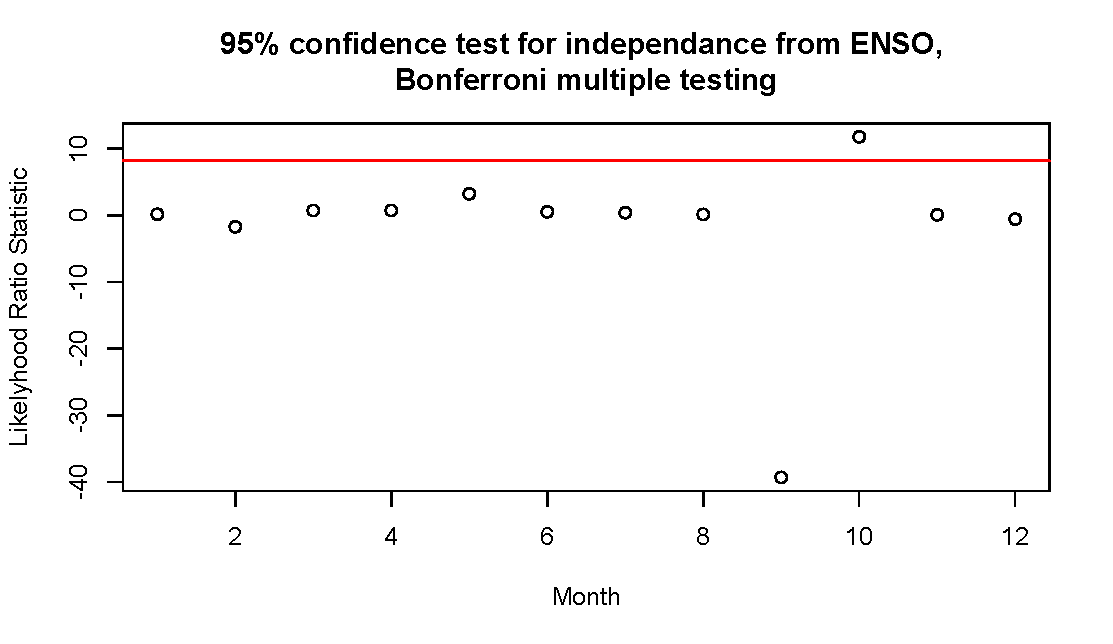
\includegraphics[width=0.35\textwidth]{../plots/enso_dependance.pdf}\\
	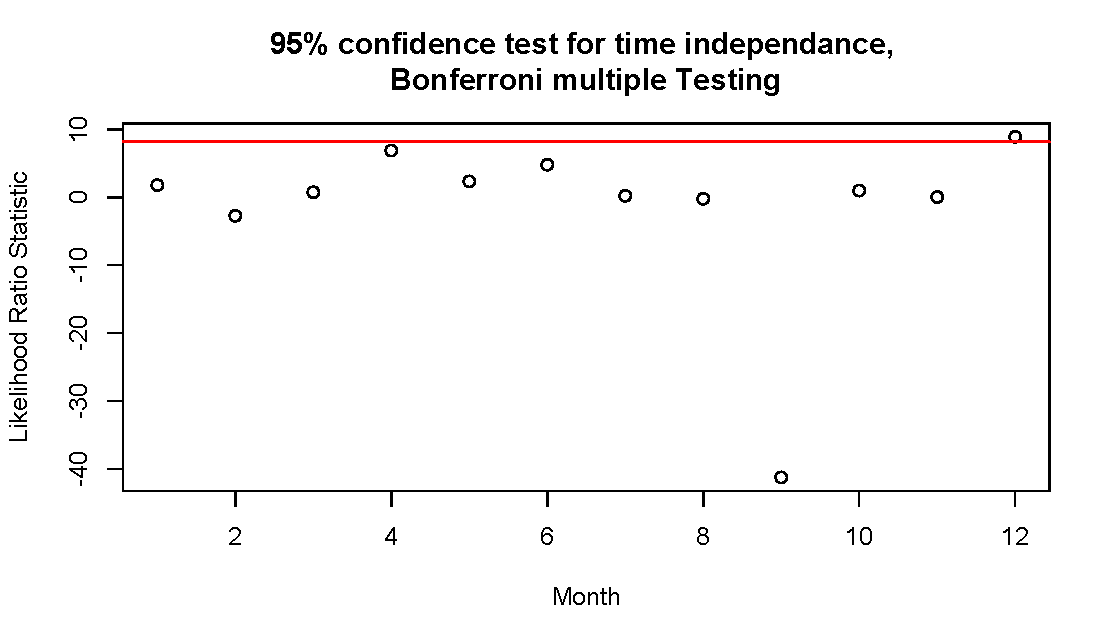
\includegraphics[width=0.35\textwidth]{../plots/time_dependance.pdf}
	\caption{Plots for likelihood ratios and 95\% significance levels for linear dependence}
	\label{fig:dependance_test}
\end{figure}

\begin{figure}
	\centering
	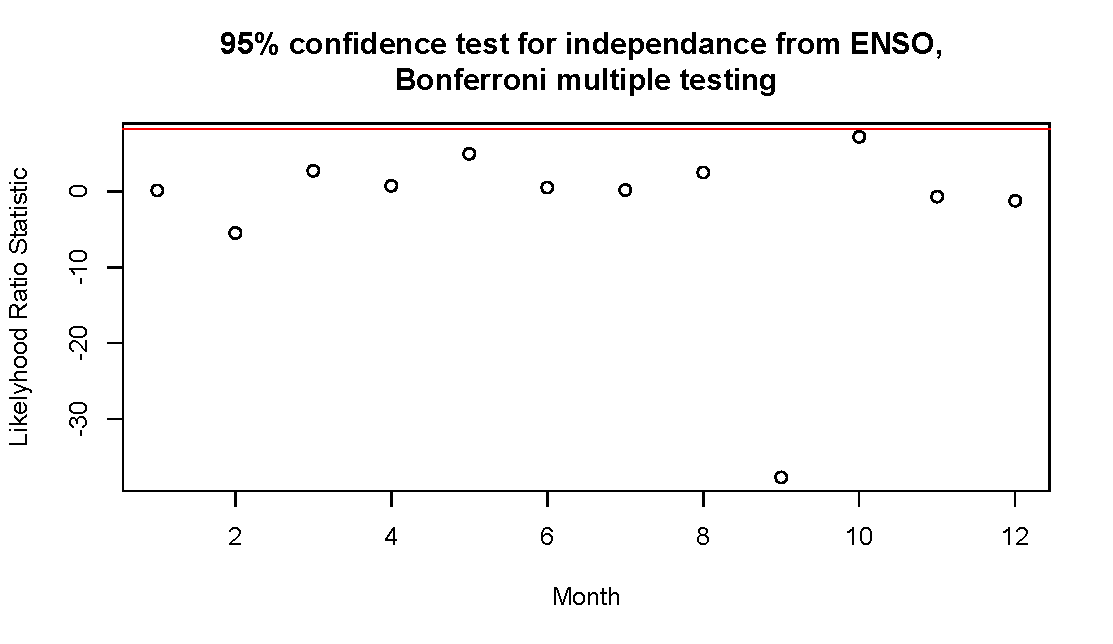
\includegraphics[width=0.35\textwidth]{../plots/enso_dependance_step.pdf}\\
	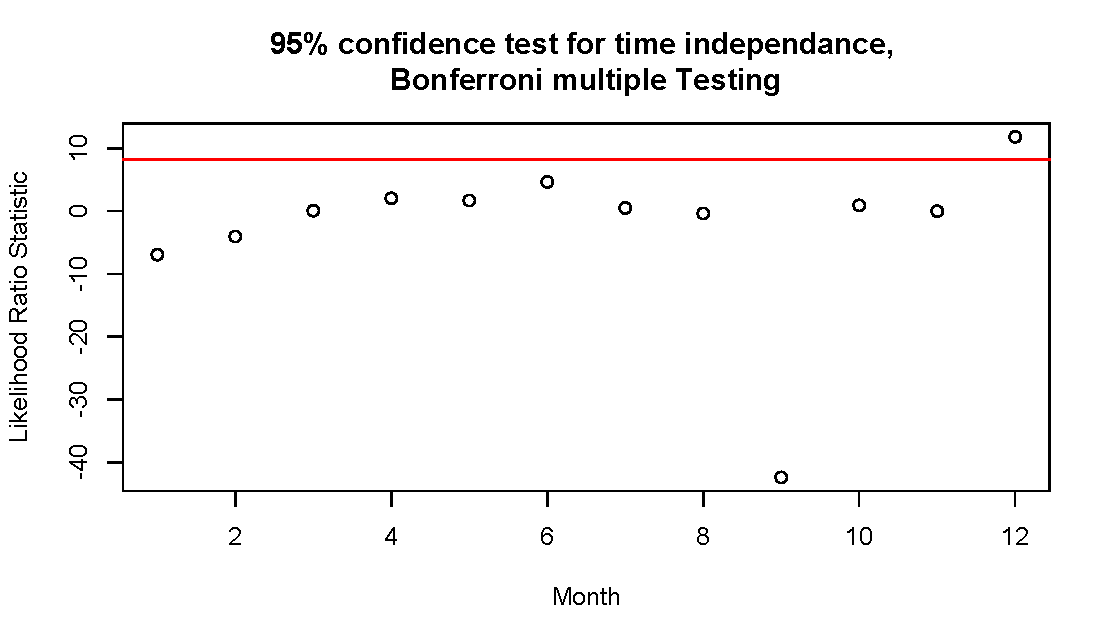
\includegraphics[width=0.35\textwidth]{../plots/time_dependance_step.pdf}
	\caption{Plots for likelihood ratios and 95\% significance levels for step dependence}
	\label{fig:dependance_test_step}
\end{figure}
\section*{Clustering of Extremes}
The general theory for the GEV is under the assumption that the samples are independent. If dependence is present, we can estimate the clustering using the extremal index $\theta$. There are many interpretations of the extremal index, we will only give 2 here. An intuitive interpretation is that $\theta^{-1}$ is the mean limiting size of the clusters of threshold exceedances. For a more mathematical interpretation, let $\{X_i\}$ be a stationary process and let  $\{X_i^*\}$ be independent variables with the same marginal distribution. If the maxima of the $X_i$ have a limiting distribution $H(z)$ and the maxima of $X_i^*$ have a limiting distribution $H^*(z)$, then it can be shown that $H(z)=H^*(z)^\theta$. Since $\eta=\eta^*-\tau^*\frac{1-\theta^\xi}{\xi}\leq\eta^*$, the maxima of the independent variables have bigger extremes than the maxima of the dependent processes. 
\par
Figure \ref{fig:extremal_index} shows the extremal indexes for every month. Since they are smaller than one, some clustering does occur. This would affect the analysis of $r$-largest order statistics as well as peak-over-threshold analysis. However, models using monthly maxima aren't affected since they rely on only one value per month, making clustering irrelevant. Moreover, we see that the clusters are bigger in summer, with average cluster sizes of 4, in winter the average cluster sizes are more in the region of 2. This indicates that the necessary conditions for extreme thunderstorms are given for a longer time during summer, possibly also leading to longer-during thunderstorms than in winter. 
%TODO: SCHRIBE DAS R LARGEST SCHLECHT ISCH

\begin{figure}
	\centering
	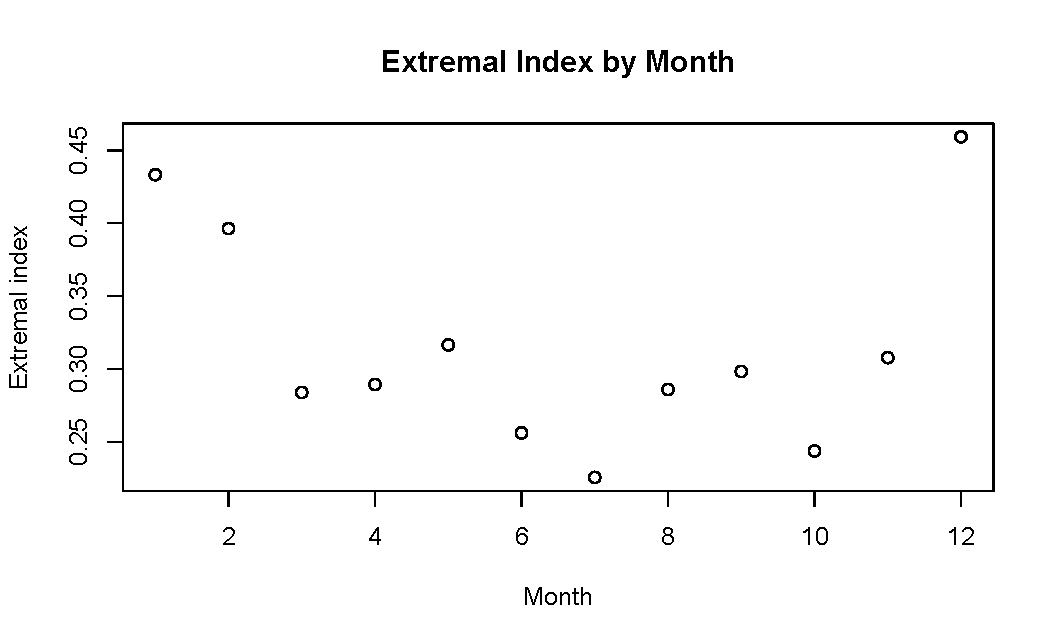
\includegraphics[width=0.35\textwidth]{../plots/extermal_index.pdf}
	\caption{Extremal index estimation using evd function exi}
	\label{fig:extremal_index}
\end{figure}


\section*{Approach to Analysing Annual Maxima for all Months Together}
In our analysis, we have clearly seen that there is seasonality in the data. If we would have to fit a distribution to a dataset without splitting the months, the best approach in our opinion would be to account for this seasonality by including a seasonal parameter (sinusoidal) in $\eta$, such that the location parameter would be estimated by $\eta = \eta_0 + \eta_1*x$, where $x$ is a seasonality trend. For example we could take $x=cos(\frac{2\pi m}{12}-\alpha)$, where $m$ is the month index and $\alpha$ is an appropriate shift. The problem would be that while we do incorporate seasonality in the location parameter, we don't in the scale and shape parameter. The obvious strength of this approach would be that we could make inference about the annual maxima and their return levels. Also, we would have 12 times as many data points, which would be a substantial improvement from the only 37 samples we have now (for monthly maxima).
\par
We believe that it would be possible however, to estimate annual maxima and their return levels from our analysis above. For this, we would propose sampling extremes for each month, and then estimate return levels for the annual maxima. This approach is similar to what we incorporate for the return level calculation with the bivariate fit.


\section*{Dependence of CAPE and SRH}
Asymptotic dependence (or independence) of bivariate maxima of two random variables can be estimated using $\chi$ and $\bar{\chi}$ plots as provided by the \texttt{chiplot} function of the \texttt{evd} package \cite{evd}. The $\chi$ plot estimates for two random variables, $X \sim F_X$ and $Y \sim F_Y$, the probability 
\begin{align*}
	P\{F_X (X) > u | F_Y (Y) > u\}
\end{align*}
for a given probability threshold $u$. The asymptotic behavior is observed as the upper support point of the distributions are attained, as $u \to 1$. If the maxima are independent, the quantity $\lim_{u \to 1} \chi(u) = 0$. Whereas $\chi(u)$ can measure the strength of the dependence, the rate at which $\chi(u) \to 0$ as $u \to 1$ is measured by the $\bar{\chi}$ plot. Generally we can say that for asymptotic independence $\lim_{u \to 1} \bar{\chi}(u) \to 0$, and for asymptotic dependence $\lim_{u \to 1} \bar{\chi}(u) \to 1$. 
%The value of interest is $\chi = \lim_{u \to 1} \chi(u)$. For independence, $\chi \to 0$, since as $u \to 1$, $P\{F_X(x)>u | F_Y(y)>u\} \to \chi$. $\chi$ can distinguish the strength of dependence, but not the rate at which $\chi(u) \to 0$ as $u \to 1$. For this we can use the $\bar{\chi}$ plot. Generally we can say that for asymptotic independence $\lim_{u \to 1} \bar{\chi}(u) \to 0$, and for asymptotic dependence $\lim_{u \to 1} \bar{\chi}(u) \to 1$. (Source Slides 239-242 of the lecture notes)
\par
Our chi plots for all months look very similar. They suggest asymptotic independence between $CAPE$ and $SRH$ since $\lim_{u \to 1} \chi(u) \to 0$ and $\lim_{u \to 1} \bar{\chi}(u) \to 0$. Figure \ref{fig:cape_srh_chi} shows two representative examples of $\chi$ and $\bar{\chi}$ plots, for May and November. 

\begin{figure}
	\centering
	\textbf{May}\\
	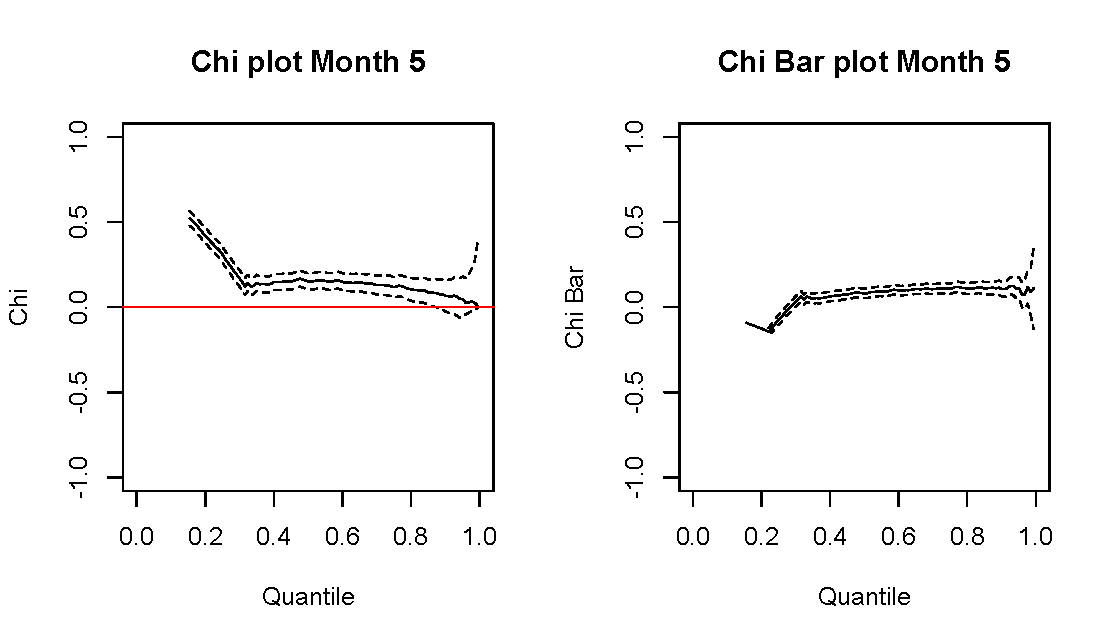
\includegraphics[width=0.35\textwidth]{../plots/May_chi.pdf}\\
	\textbf{November}\\
	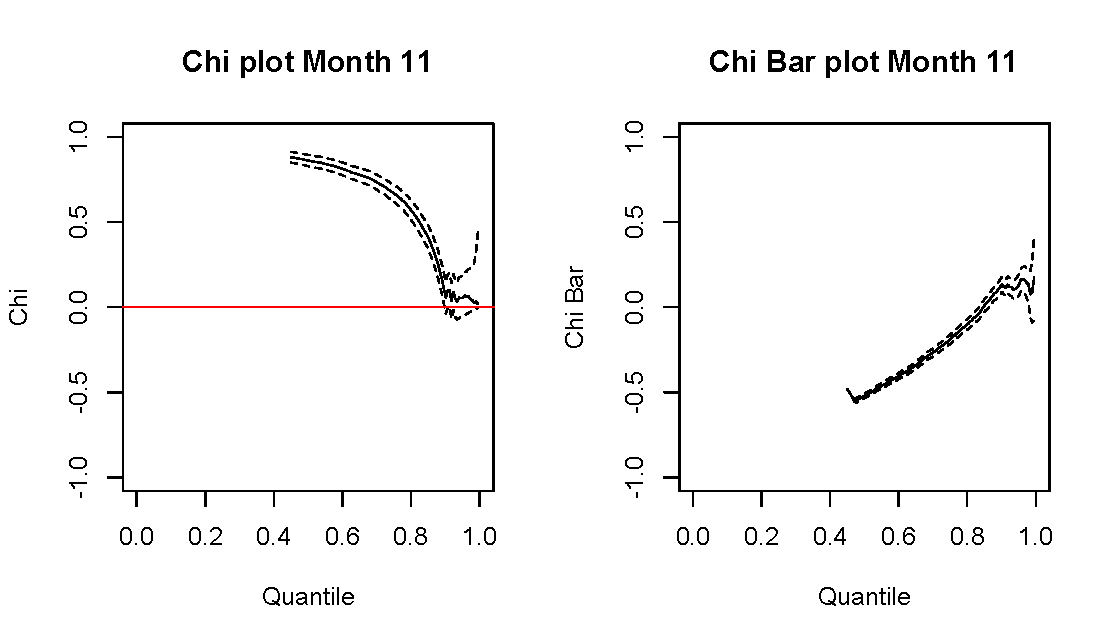
\includegraphics[width=0.35\textwidth]{../plots/November_chi.pdf}
	\caption{Representative examples for chi plots for $CAPE$ and $SRH$, both suggesting asymptotic independence since they approach 0 as the quantile $u \to 1$.}
	\label{fig:cape_srh_chi}
\end{figure}

\section*{Bivariate Fitting of CAPE and SRH}
Whereas until now only the single structure variable $PROD$ was considered, in this section its two components $CAPE$ and $SRH$ are taken separately. A bivarate extreme value distribution is  fitted to the data with the \texttt{fbvevd} function of the \texttt{evd} package \cite{evd}, using six different parametric link functions. The tested link functions were logistic (log), asymmetric logistic (alog), negative logistic (neglog), bilogistic (bilog), Coles-Tawn (ct) and negative bilogistic models (negbilog), and thus comprised symmetric and asymmetric models. The quality of the fit using different link functions were compared using the Akaike Information Criterion (AIC), as shown in Table \ref{table:cape_srh_AIC}.
\par
We observe that the negative logistic link function is the best or among the best fits for all months. This suggests that the introduction of asymmetry between $CAPE$ and $SRH$ doesn't improve the fit. In order to treat all months consistently, fits using this link function for all months were used for subsequent analysis. 
\begin{table}[]
\begin{tabular}{lllllll}
Month     & log       & alog      & neglog    & bilog     & ct        & negbilog  \\
January   & 920.4  & 921.3  & 920.1  & 920.3  & 921.0  & 920.3  \\
February  & 993.3  & 997.1  & 993.5  & 995.3  & 996.2  & 994.8  \\
March     & 1070.1 & 1074.2 & 1069.5 & 1072.2 & 1074.1 & 1071.6 \\
April     & 1064.8 & 1068.7 & 1064.6 & 1066.1 & 1066.2 & 1066.3 \\
May       & 1066.5 & 1070.4 & 1066.5 & 1068.3 & 1071.0 & 1068.2 \\
June      & 1043.3 & 1047.0 & 1043.4 & 1040.7 & 1043.1 & 1045.5 \\
July      & 1047.0 & 1044.9 & 1046.7 & 1046.2 & 1048.4 & 1046.5 \\
August    & 1029.2 & 1033.0 & 1029.4 & 1031.1 & 1031.3 & 1031.2 \\
September & 1056.0 & 1059.6 & 1055.7 & 1058.1 & 1059.9 & 1057.3 \\
October   & 1038.0 & 1042.0 & 1037.6 & 1037.6 & 1039.3 & 1038.5 \\
November  & 1012.4 & 1016.4 & 1012.7 & 1014.5 & 1015.1 & 1014.1 \\
December  & 892.7  & 896.7  & 892.5  & 894.9  & 895.5  & 894.3
\end{tabular}
\caption{AIC comparison of different link function models}
\label{table:cape_srh_AIC}
\end{table}
Note that for this fit, we extracted for each month the maximal $SRH$ value and the maximal $CAPE$ value and fitted the distribution to this data pair. However, the monthly maximum of these two independent variables don't necessarily correspond to the same event. We have therefore to be careful when drawing conclusions, since the "observations" we fit the models to often don't actually exist.
\par
Before, we estimated the dependence between $CAPE$ and $SRH$. We can also these results with the fits we just made. For this we will use the dependence parameter $r$ from the negative logistic model. This positive parameter tends to infinity for dependence, and to zero for independence. In Figure \ref{fig:cape_srh_dependance_logistic} we plot the dependence parameters for every month with crude estimates of 95\% confidence bands using the standard error of the parameter. Since all of the dependence parameters are close to zero, independence cannot be ruled out. 

\begin{figure}
	\centering
	\includegraphics[width=0.35\textwidth]{../plots/monthly_dependence.pdf}
	\caption{Monthly dependence parameter $r$ with 95\% confidence intervals, compared to independence ($r=0$)}
	\label{fig:cape_srh_dependance_logistic}
\end{figure}

\section*{Calculation of Return Levels}
The return levels of extreme events is a quantity of interest for risk assessment. Here, we estimate the return levels using the different estimated fits obtained above. Notably, we compare 50- and 100 year return levels of $PROD$ using the location $\hat{\nu}$, scale $\hat{\tau}$ and shape $\hat{\xi}$ estimates obtained above for every month using maximum likelihood estimation (MLE), Bayesian fitting (BAY), the $r$-largest order statistics (LAR). 
\par
We also obtain the return levels using a Poisson process approach (POI): %TODO ????????
\par
Additionally, we compute return levels based on the bivariate fit as follows (BIV): Using the function \texttt{rbvevd} from the \texttt{evd} package, we simulate 500'000 observations of $SRH$ and $CAPE$ using the fitted distribution obtained above with the negative logarithmic link function. We then calculate the resulting $PROD$ value of the simulated observation pairs. From this, we obtain the $n$-year return level as the $1-1/n$ quantile. 
\par
% TODO: RETURN LEVEL
The results in Figure \ref{fig:return_lvl} that the values obtained using the Poisson process approach correspond well with the Bayesian results. Both show a seasonal trend for both the 50-year and 100-year return levels, with values in spring and the lowest during late fall and winter. The Bayesian results seem to be more smooth throughout the year, which probably more realistic than high fluctuations between months. 
\par
Return levels estimated with the bivariate fit are generally higher than the others. This is likely due to the problematic discussed above, that simultaneous monthly maxima of $CAPE$ and $SRH$ are simulated. Since the maxima of these two values don't necessarily occur simultaneously, as illustrated by their asymptotic independence, we simulate values of $PROD$ that overestimate the actual values. Hence, the return levels obtained this way likely overestimate the ground truth. Similar seasonality is observed as in the case of the other results. 
\par
While the different models yield consistent seasonality results in general, a discrepancy is observed in January and February for the 100 year levels which are estimated as being the highest by BIV. In contrast, the values in January are among the lowest for both the BAY and POI, whereas February is also low for BAY, while it is the highest for POI. % TODO WIESO??? 

\section*{Impact by Using Variable Transformations}
We argue (without testing this explicitly), that using a $log(\cdot)$ transformation on $CAPE$, $SRH$ and $PROD$ would not change our analysis much. If $CAPE$ and $SRH$ arise from a joint distribution $F$, then $log(CAPE)$ and $log(SRH)$ arise from a distribution $F'$. The \textit{Extremal Types Theorem} (Seen on slide 31 of the course) shows that if a limiting extremal distribution exists, it must be the GEV. Since the $log(\cdot)$ operation maps values $x>1$ to $log(x)<x$, the upper tails will be lighter and the distribution will exist. The dependence analysis would yield different results: Since if the shape parameter has linear dependence in log space, it has exponential dependence in linear space. To do the same analysis, we would have to use a transformed trend $x_{new}= log(x)$. 

\section*{Conclusion}
We have analysed the thunderstorm risk using several methods from the toolbox of extremal analysis. The key insights are that, in accordance with common knowledge, the thunderstorm risk is greater in summer than in winter. Also, we cannot conclude that the shape parameter $\xi$ is negative, suggesting that there is no upper limit in the strength of thunderstorms for the region analysed in this report.
\par
We have also compared different fitting methods, and seen their strengths and weaknesses. We saw that if we are aware of the weakness of the method we apply, we can better understand the fit, as the possible errors can easily be spotted. 
\par
A clear deficit of the analysis performed in this report is the lack of data: When treating every month differently and taking monthly maxima, we relied on only 37 data points for model fitting. One way to better model the thunderstorm behavior would be using spatial extremes, by taking into account data measured at other locations. This would yield more data, but could also reveal interesting behavior of extreme thunderstorm formation, possibly giving valuable physical insight. 


%%% Bibliography
\bibliographystyle{IEEEtran}
\bibliography{literature-project}


% TODO:
% Explain why discrepancy
% Schribe das r-largest eue schlecht isch
% Parameter vergliiche vode verschidnige fitting methode
% Poisson process approach
% Bibliographie!!!


\end{document}
